\documentclass[11pt]{article}
\usepackage[textwidth=18.0cm, textheight=23.0cm, top=2.0cm]{geometry}
\usepackage{pst-all}
\usepackage{amssymb}
\usepackage{tikz}
\usepackage{underscore}\begin{document}
\pagestyle{empty}


ClassName: \underline{\textbf{Class_07.2bp-4}}
\par
BinSize: \underline{\textbf{100 × 100}}
\par
ReduceSize: \underline{\textbf{100 × 99}}
\par
TypeNum: \underline{\textbf{20}}
\par
Num: \underline{\textbf{20}}
\par
OutS: \underline{\textbf{60000}}
\par
InS: \underline{\textbf{46202}}
\par
Rate: \underline{\textbf{0.770}}
\par
UB: \underline{\textbf{6}}
\par
LB0: \underline{\textbf{6}}
\par
LB: \underline{\textbf{6}}
\par
LBWithCut: \underline{\textbf{6}}
\par
NodeCut: \underline{\textbf{0}}
\par
ExtendedNodeCnt: \underline{\textbf{1}}
\par
GenNodeCnt: \underline{\textbf{1}}
\par
PrimalNode: \underline{\textbf{0}}
\par
ColumnCount: \underline{\textbf{6}}
\par
TotalCutCount: \underline{\textbf{0}}
\par
RootCutCount: \underline{\textbf{0}}
\par
LPSolverCnt: \underline{\textbf{1}}
\par
PricingSolverCnt: \underline{\textbf{0}}
\par
BranchAndBoundNum: \underline{\textbf{1}}
\par
isOpt: \underline{\textbf{true}}
\par
TimeOnInitSolution: \underline{\textbf{0.000 s}}
\par
TimeOnPrimal: \underline{\textbf{0.000 s}}
\par
TimeOnPricing: \underline{\textbf{0.000 s}}
\par
TimeOnRmp: \underline{\textbf{0.062 s}}
\par
TotalTime: \underline{\textbf{0.125 s}}
\par
\newpage


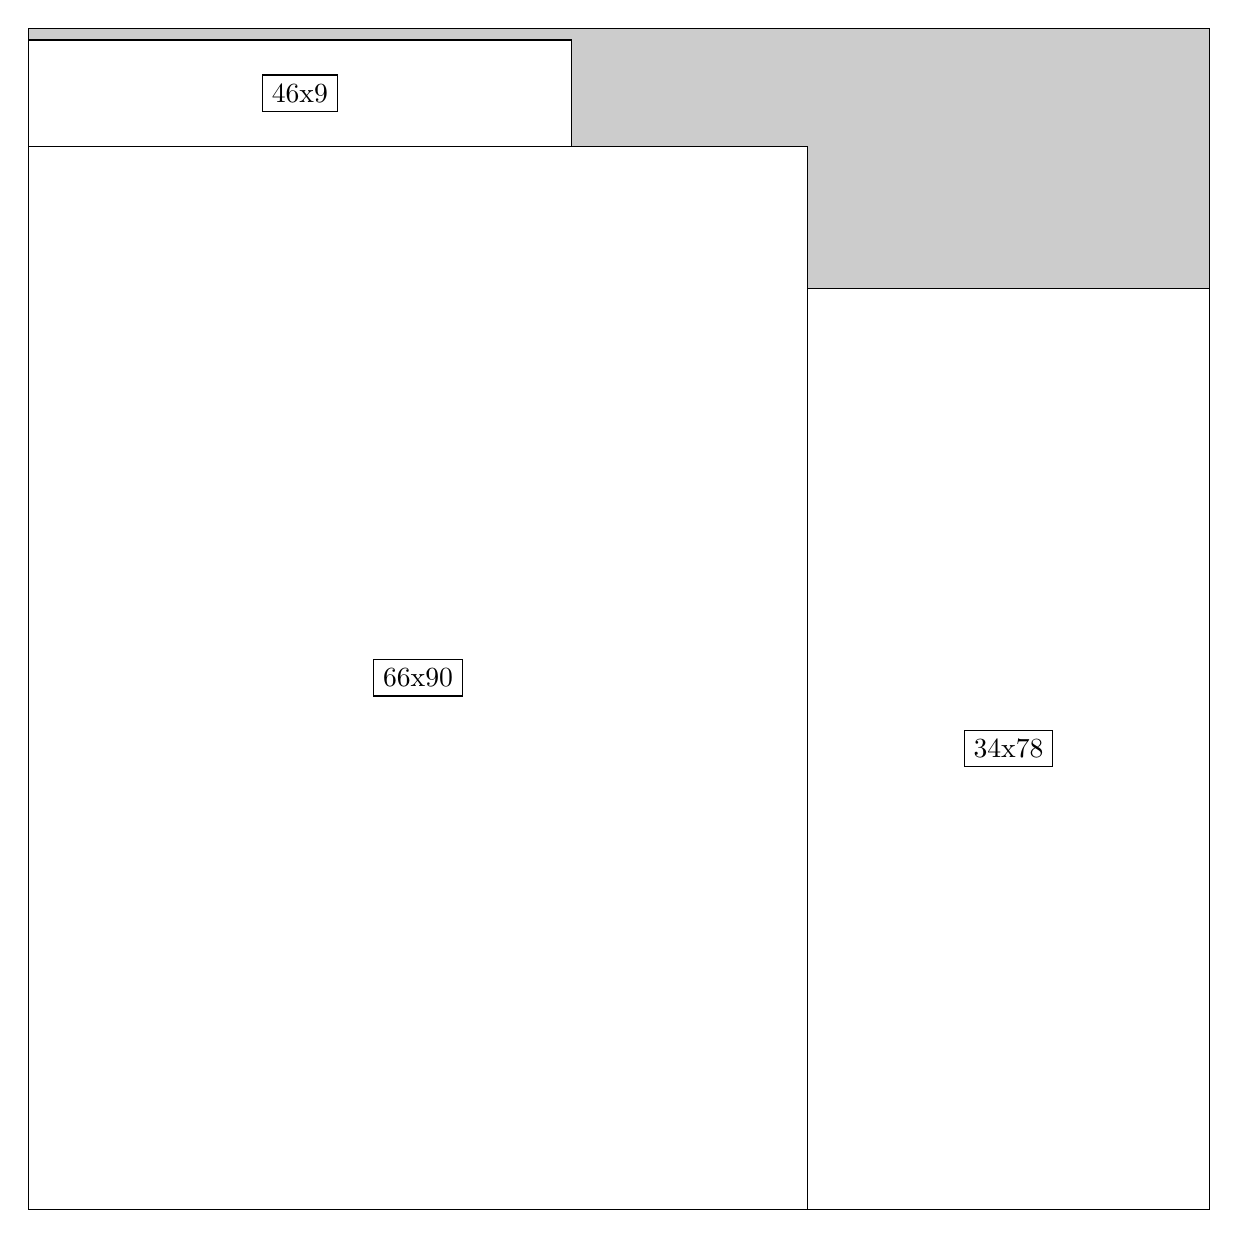
\begin{tikzpicture}[shorten >=1pt,scale=1.0,every node/.style={scale=1.0},->]
\tikzstyle{vertex}=[circle,fill=black!25,minimum size=14pt,inner sep=0pt]
\filldraw[fill=gray!40!white, draw=black] (0,0) rectangle (15.0,15.0);
\foreach \name/\x/\y/\w/\h in {66x90/0.0/0.0/9.9/13.5,34x78/9.9/0.0/5.1/11.7,46x9/0.0/13.5/6.8999999999999995/1.3499999999999999}
\filldraw[fill=white!40!white, draw=black] (\x,\y) rectangle node[draw] (\name) {\name} ++(\w,\h);
\end{tikzpicture}


w =66 , h =90 , x =0 , y =0 , v =5940
\par
w =34 , h =78 , x =66 , y =0 , v =2652
\par
w =46 , h =9 , x =0 , y =90 , v =414
\par
\newpage


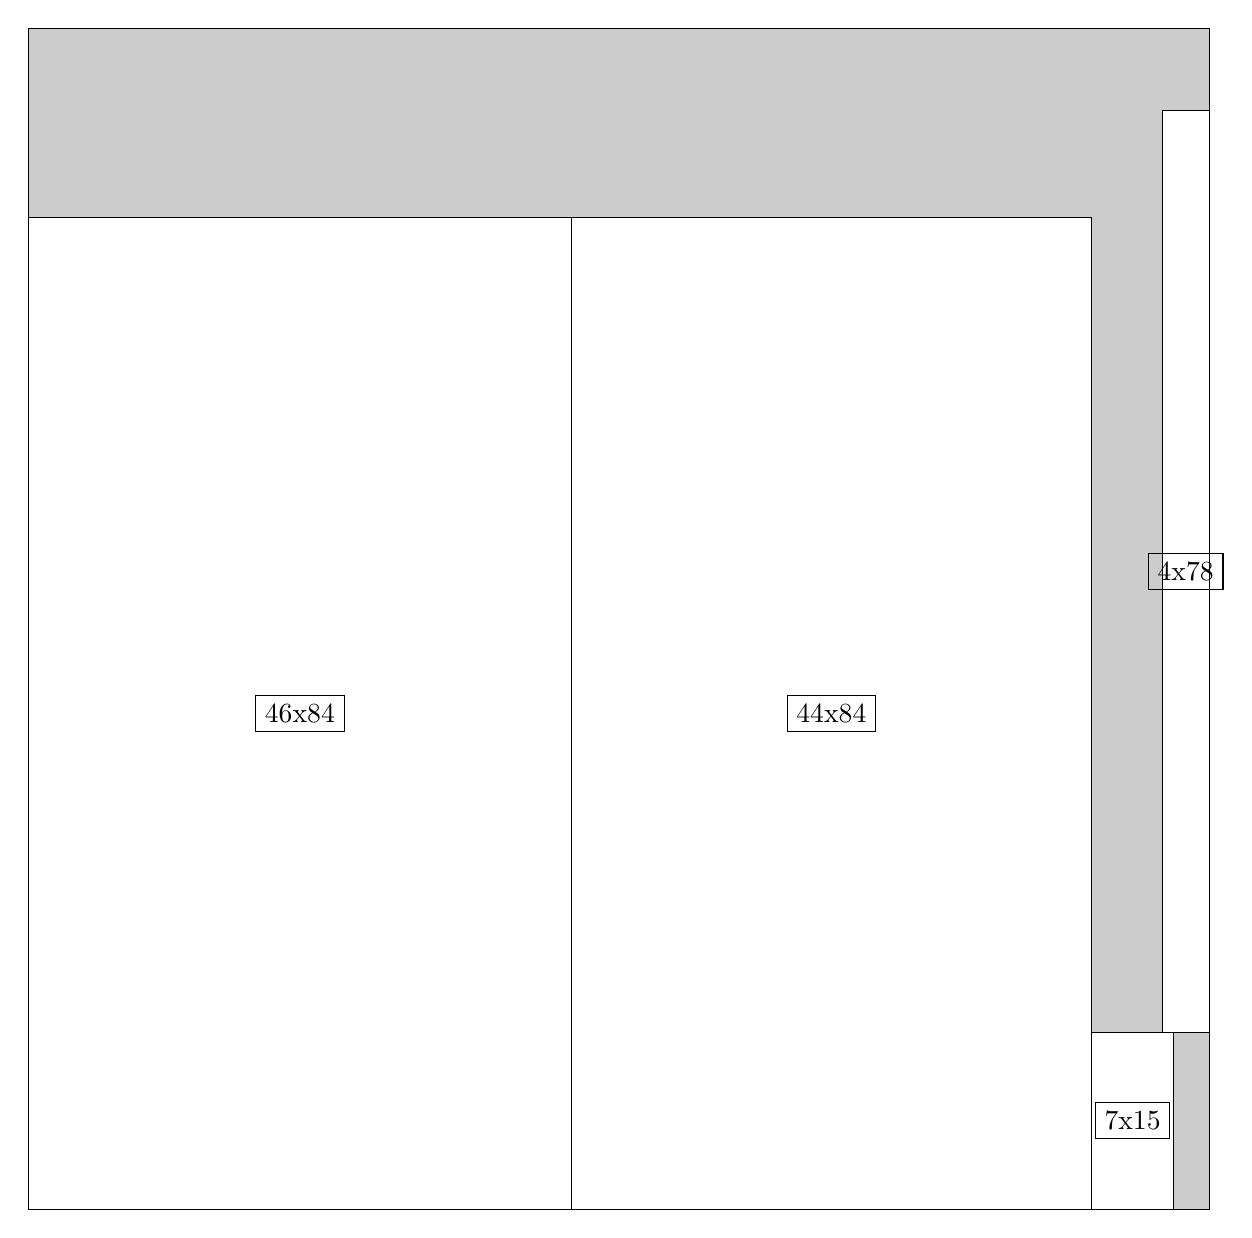
\begin{tikzpicture}[shorten >=1pt,scale=1.0,every node/.style={scale=1.0},->]
\tikzstyle{vertex}=[circle,fill=black!25,minimum size=14pt,inner sep=0pt]
\filldraw[fill=gray!40!white, draw=black] (0,0) rectangle (15.0,15.0);
\foreach \name/\x/\y/\w/\h in {46x84/0.0/0.0/6.8999999999999995/12.6,44x84/6.8999999999999995/0.0/6.6/12.6,4x78/14.399999999999999/2.25/0.6/11.7,7x15/13.5/0.0/1.05/2.25}
\filldraw[fill=white!40!white, draw=black] (\x,\y) rectangle node[draw] (\name) {\name} ++(\w,\h);
\end{tikzpicture}


w =46 , h =84 , x =0 , y =0 , v =3864
\par
w =44 , h =84 , x =46 , y =0 , v =3696
\par
w =4 , h =78 , x =96 , y =15 , v =312
\par
w =7 , h =15 , x =90 , y =0 , v =105
\par
\newpage


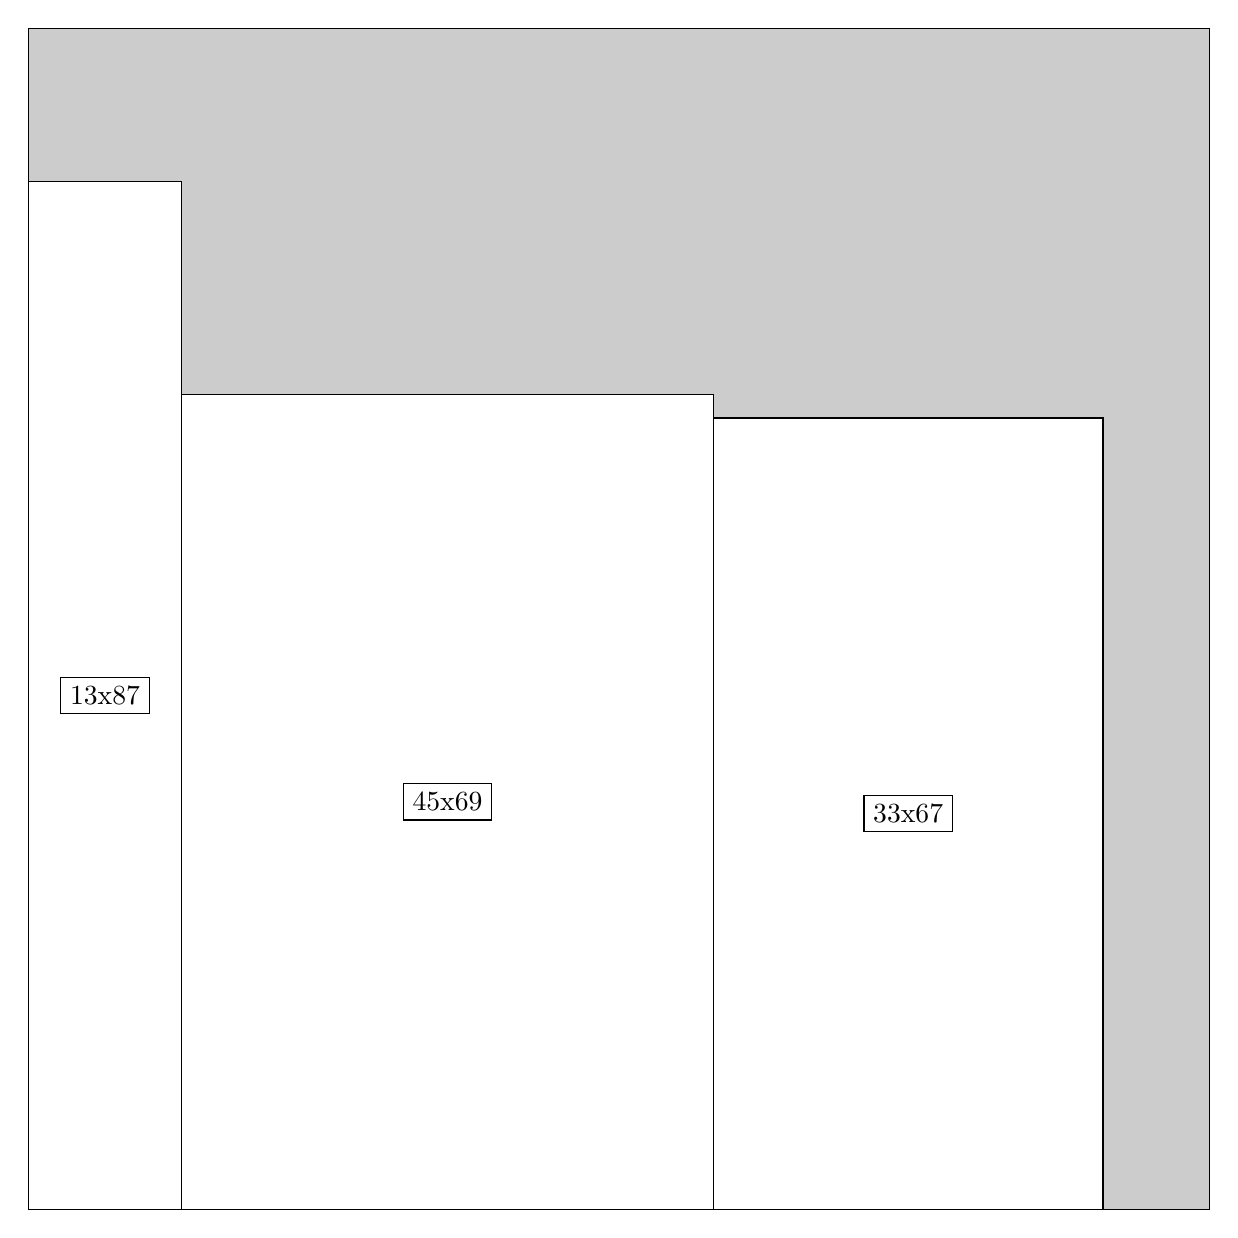
\begin{tikzpicture}[shorten >=1pt,scale=1.0,every node/.style={scale=1.0},->]
\tikzstyle{vertex}=[circle,fill=black!25,minimum size=14pt,inner sep=0pt]
\filldraw[fill=gray!40!white, draw=black] (0,0) rectangle (15.0,15.0);
\foreach \name/\x/\y/\w/\h in {13x87/0.0/0.0/1.95/13.049999999999999,45x69/1.95/0.0/6.75/10.35,33x67/8.7/0.0/4.95/10.049999999999999}
\filldraw[fill=white!40!white, draw=black] (\x,\y) rectangle node[draw] (\name) {\name} ++(\w,\h);
\end{tikzpicture}


w =13 , h =87 , x =0 , y =0 , v =1131
\par
w =45 , h =69 , x =13 , y =0 , v =3105
\par
w =33 , h =67 , x =58 , y =0 , v =2211
\par
\newpage


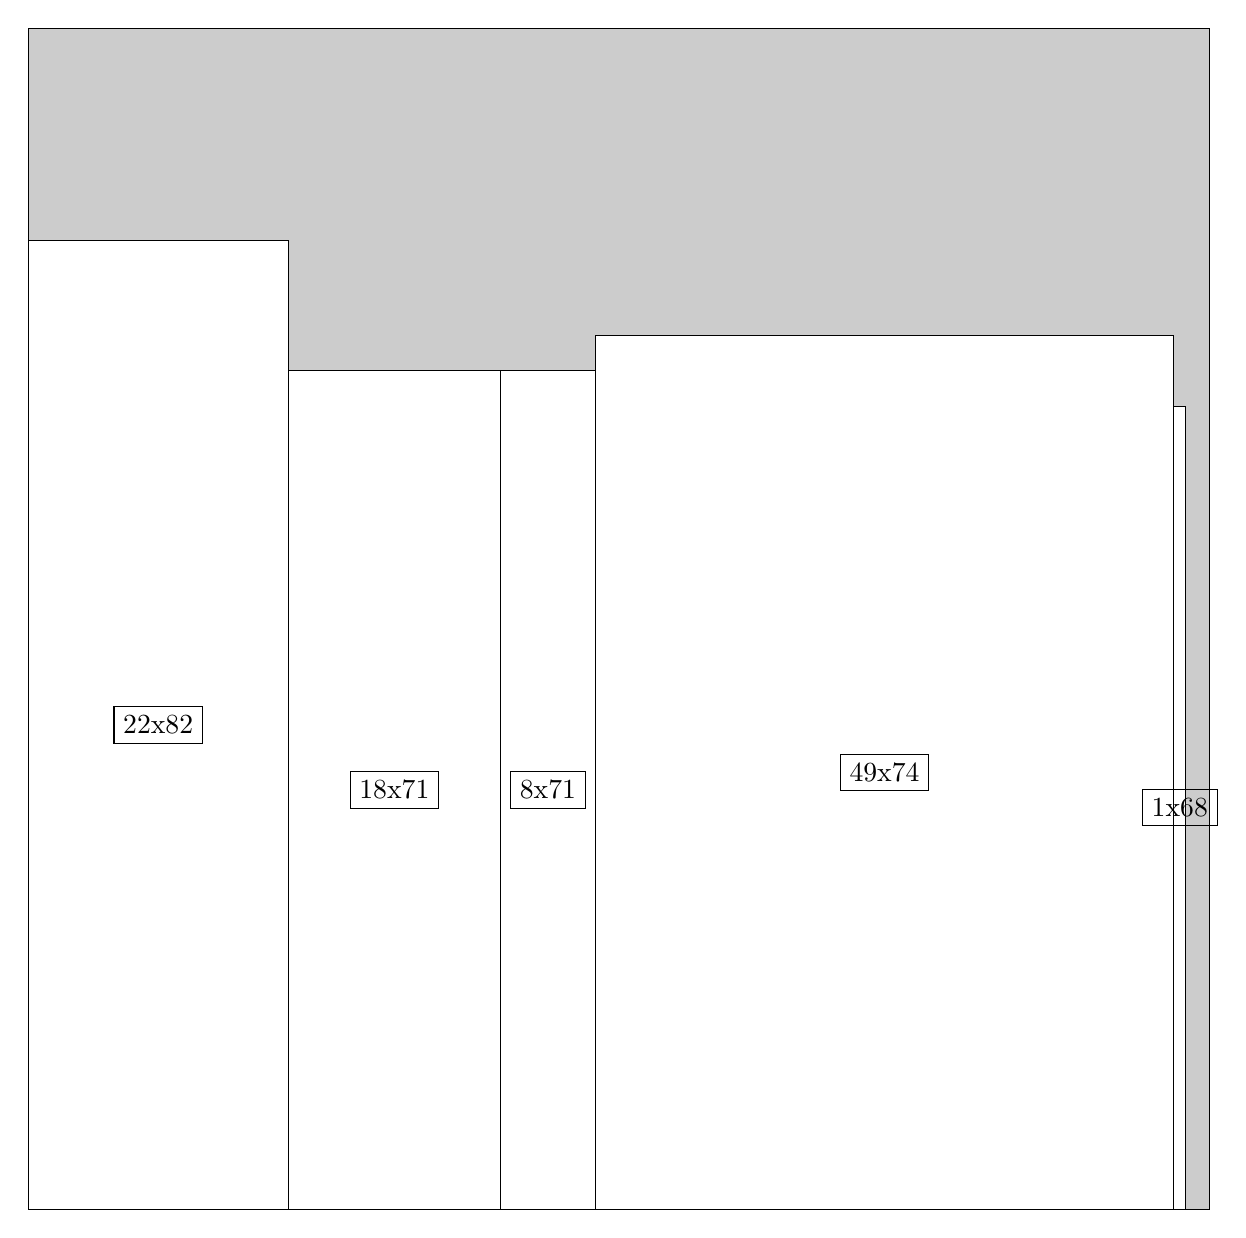
\begin{tikzpicture}[shorten >=1pt,scale=1.0,every node/.style={scale=1.0},->]
\tikzstyle{vertex}=[circle,fill=black!25,minimum size=14pt,inner sep=0pt]
\filldraw[fill=gray!40!white, draw=black] (0,0) rectangle (15.0,15.0);
\foreach \name/\x/\y/\w/\h in {22x82/0.0/0.0/3.3/12.299999999999999,18x71/3.3/0.0/2.6999999999999997/10.65,49x74/7.199999999999999/0.0/7.35/11.1,8x71/6.0/0.0/1.2/10.65,1x68/14.549999999999999/0.0/0.15/10.2}
\filldraw[fill=white!40!white, draw=black] (\x,\y) rectangle node[draw] (\name) {\name} ++(\w,\h);
\end{tikzpicture}


w =22 , h =82 , x =0 , y =0 , v =1804
\par
w =18 , h =71 , x =22 , y =0 , v =1278
\par
w =49 , h =74 , x =48 , y =0 , v =3626
\par
w =8 , h =71 , x =40 , y =0 , v =568
\par
w =1 , h =68 , x =97 , y =0 , v =68
\par
\newpage


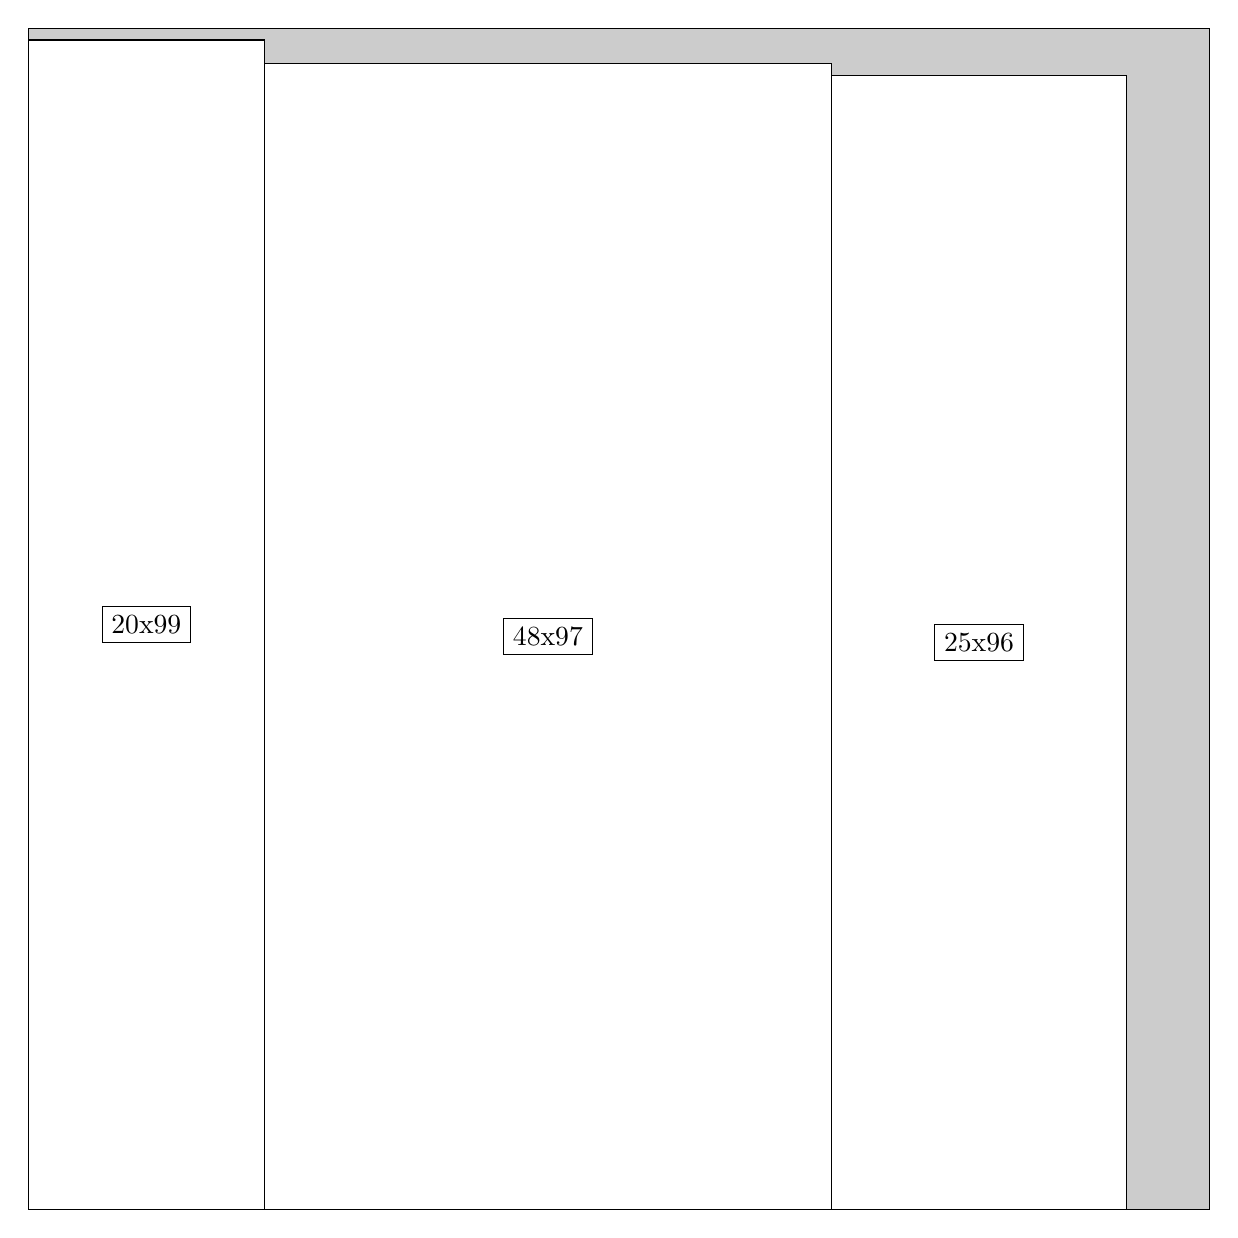
\begin{tikzpicture}[shorten >=1pt,scale=1.0,every node/.style={scale=1.0},->]
\tikzstyle{vertex}=[circle,fill=black!25,minimum size=14pt,inner sep=0pt]
\filldraw[fill=gray!40!white, draw=black] (0,0) rectangle (15.0,15.0);
\foreach \name/\x/\y/\w/\h in {48x97/3.0/0.0/7.199999999999999/14.549999999999999,25x96/10.2/0.0/3.75/14.399999999999999,20x99/0.0/0.0/3.0/14.85}
\filldraw[fill=white!40!white, draw=black] (\x,\y) rectangle node[draw] (\name) {\name} ++(\w,\h);
\end{tikzpicture}


w =48 , h =97 , x =20 , y =0 , v =4656
\par
w =25 , h =96 , x =68 , y =0 , v =2400
\par
w =20 , h =99 , x =0 , y =0 , v =1980
\par
\newpage


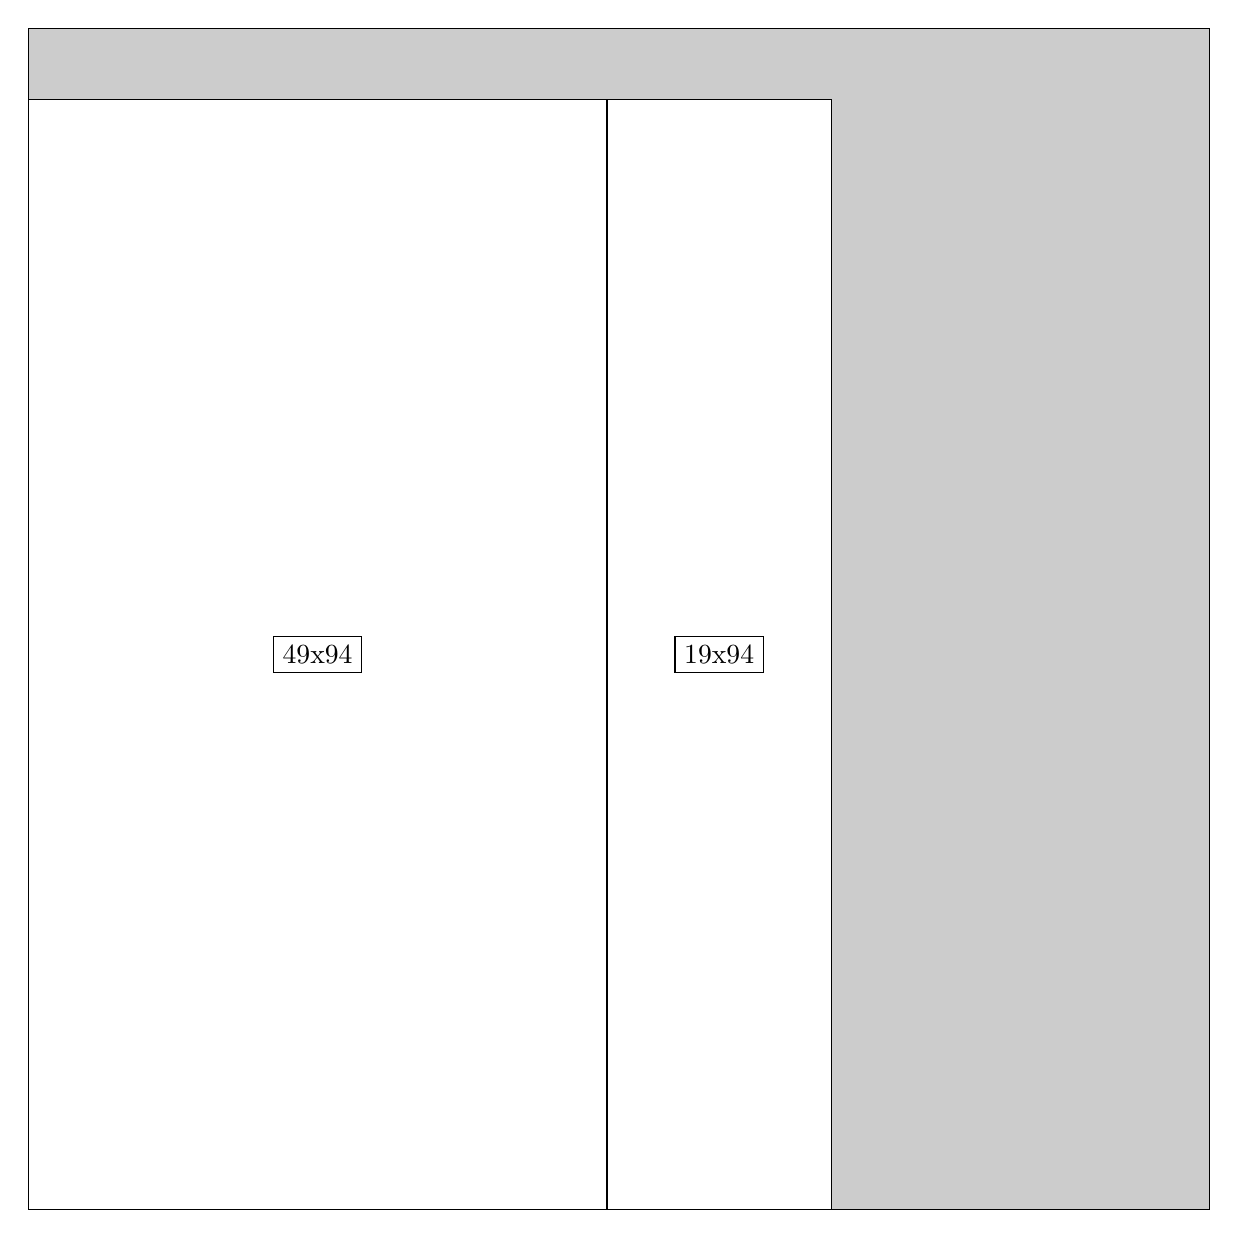
\begin{tikzpicture}[shorten >=1pt,scale=1.0,every node/.style={scale=1.0},->]
\tikzstyle{vertex}=[circle,fill=black!25,minimum size=14pt,inner sep=0pt]
\filldraw[fill=gray!40!white, draw=black] (0,0) rectangle (15.0,15.0);
\foreach \name/\x/\y/\w/\h in {49x94/0.0/0.0/7.35/14.1,19x94/7.35/0.0/2.85/14.1}
\filldraw[fill=white!40!white, draw=black] (\x,\y) rectangle node[draw] (\name) {\name} ++(\w,\h);
\end{tikzpicture}


w =49 , h =94 , x =0 , y =0 , v =4606
\par
w =19 , h =94 , x =49 , y =0 , v =1786
\par
\newpage


\end{document}